\chapter{Инструменты и оборудование}

\section{JTAG-адаптер}

% \input{jtag/soft}
% \input{stlink/stlink1}

\section{Отладочные платы}

Прежде чем начать работать с отдельными \mk, устанавливая их на плату
собственной разработки, для быстрого старта используют \term{отладочные
платы}\note{development board, demo board}

\subsection{Arduino /Atmel Mega AVR8/}

\subsection{Cortex-Mx} См. \ref{devkitcmx}

\subsection{CubieBoard /Cortex-A8 AllWinner A10/}

\subsection{Raspberry Pi /ARM11 BCM3032/}

\subsection{BlackSwift /MIPS/}

\subsection{VoCore /MIPS/}

\section{Монтажный инструмент}

\section{Измерительное оборудование}

\subsection{Тестер}

\subsection{Осциллограф}

\subsection{Логический анализатор}

\subsection{Генератор сигналов}

\subsection{Рыльцеметр}

\clearpage
\section{Электроинструмент}

\subsection{Дрелъ}

\noindent
\begin{tabular}{p{0.5\textwidth} p{0.5\textwidth}}
\noindent
\href{http://leroymerlin.ru/catalogue/instrumenty/elektroinstrument/dreli\_udarnye/13805983/}{
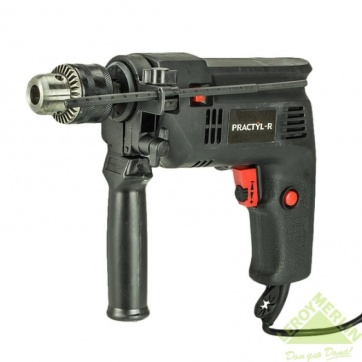
\includegraphics[width=0.45\textwidth]{../scratcher/00/fig/PraktylR.jpg}}
&
\noindent
\href{http://leroymerlin.ru/catalogue/instrumenty/elektroinstrument/dreli\_bezudarnye/11857763/}{
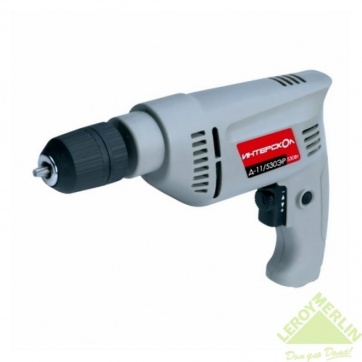
\includegraphics[width=0.45\textwidth]{../scratcher/00/fig/D_11_530ER.jpg}}
\\
\textbf{Дрель ударная сетевая} & \textbf{Дрель безударная сетевая} \\
\textbf{Praktyl-R PID13D01 400\,Вт} & \textbf{Интерскол Д-11/530ЭР (с БЗП)} \\
\textbf{(!)395\,р.} & \textbf{1120\,р.} \\
\end{tabular}

